\usepackage[utf8]{inputenc}
\usepackage[T1]{fontenc}

\usepackage[english, brazilian]{babel}
\usepackage{tikz}
\usepackage{amsmath}
\usepackage{xkeyval}
\usepackage{relsize}
\usepackage{multimedia}
\usepackage{hyperref}
\usepackage{esdiff}
\usepackage{bm}
\usepackage{csquotes}
\usepackage[style=authoryear, doi=false, url=false]{biblatex}
\usepackage{booktabs}
\usepackage{multicol}
% General settings
\usetikzlibrary{tikzmark,arrows,shapes,positioning,chains}
\usefonttheme{professionalfonts}
\hypersetup{pdfpagemode=FullScreen}

% Custom math operators
\DeclareMathOperator{\sech}{sech}

% Beamer settings
\usetheme{Copenhagen}
\setbeamertemplate{navigation symbols}{} % remove navigation symbols
\setbeamertemplate{headline}{\vskip0.95cm} % Hides navigation bar at the top
\setbeamertemplate{caption}[numbered] % Numbered captions
\setbeamertemplate{footline}{} % Hides footer

% BACKGROUND
\newif\ifusebackground
\usebackgroundtrue

\AddToHook{shipout/background}{%
	\ifusebackground
		\put(0in,-\paperheight){%
			\includegraphics[page=2,width=\paperwidth,height=\paperheight]{template-COBEQ.pdf}%
		}%
	\fi
}
